\subsection{Individual rank lists evaluation \label{sec:eval_rl}}

In this section, the goal is to find the most adapted parameters for each rank list method proposed in Chapter~\ref{sec:methods}.
After each experiment, the most convincing metrics are retained for the fusion step in Section~\ref{sec:eval_fusion}.
The results of these experiments are summarized in Section~\ref{sec:annex_retained_text_representation} in annex.

\subsubsection{Importance of the text size in stylometry}

Previous studies have shown the importance of having documents of good quality and with at least 5000 tokens to have reliable results.
Skilled authors can easily change their style to imitate others for small texts, but it becomes more difficult for larger texts~\cite{savoy_stylo}.

For this study, an experiment on the St-Jean corpus is accomplished, to show the importance of having large documents.
To test this parameter, the number of token is artificially modified by considering only the $n$ first tokens for each text, with $n$ ranging between 9000 and 250 with steps of 250 tokens.
Figure~\ref{img:degradation} shows the three metrics used (Average precision, RPrec, HPrec) over the number of tokens.
Every metric decrease over the text size, which indicate that it becomes harder to determinate documents pairs with the same author as the text size decrease.

PAN16 corpus is a difficult corpus due to its small size, thus extracting reliable features for each text to estimate each style is also a difficult task.
After multiple tests, the PAN @ CLEF 2016 corpus is not used further in this study due to its difficulty in finding reliable Stylometric clues.
For this study having standard and easier corpus is required in order to show the proposed methods.

\begin{figure}
  \centering
  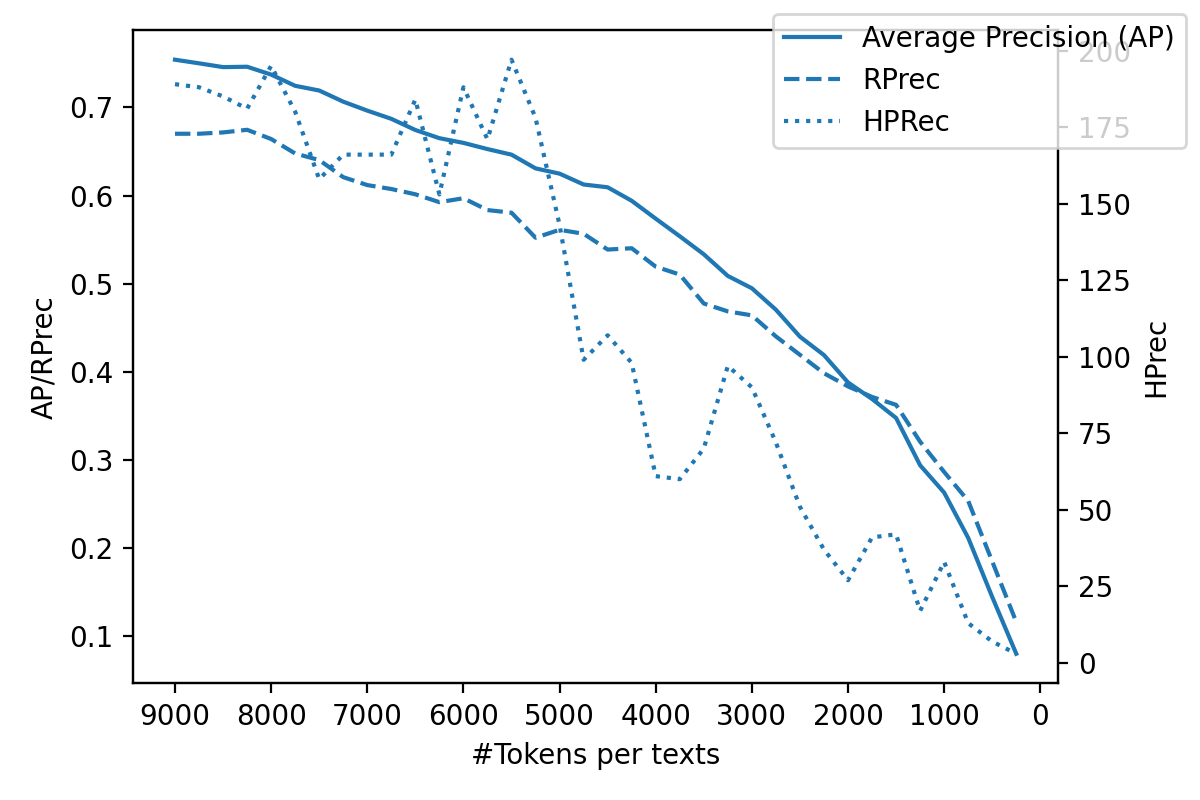
\includegraphics[width=\linewidth]{img/degradation.png}
  \caption{St-Jean ranks list evaluation on AP, RPrec and HPrec over the text size.
  Rank list computed using 500 MFW and the Z-Score normalized Cosine distance}
  \label{img:degradation}
\end{figure}

\subsubsection{MFW Token and Lemma}
\label{sec:mfw_token_lemma}

Here the goal is to compare two similar text representations, which are the token representation and the lemmatize representation.
For example \textit{il voit} (he sees) will be lemmatized to \textit{il voir} (he see).
For this kind of representation, previous studies have shown that using MFW (most frequent words) vector size of around 500 tends to produce better outcomes~\cite{savoy_text_representation}.

After creating the rank lists with the proposed distance measures (ref. Section~\ref{sec:fv_distances}) on the two representations for a MFW vector size ranging between 100 and 2000 with a step of 100, on the two datasets containing the lemmatize representation (Brunet and St-Jean), the two plots in Figure~\ref{fig:token_vs_lemma} show the average precision (AP) for the resulting rank lists.

This representation seem to have good results with a MFW vector size of 500 for most of the metrics, this corroborates previous studies results.

A few metrics, such as Manhattan distance, Tanimoto distance or Clark distance can give better results with slightly bigger vectors.
In most cases, the token representation provide on both dataset a greater average precision compared to the lemma representation.
An interesting example to be worth noticing concern the Manhattan distance, when using the token representation it tends to decrease the AP faster than the lemma representation as the MFW vector size increase.
The Euclidean distance seems to be the least appropriate distance measure for this task.
The Clark distance have a really poor average precision when the MFW vector is too small, but after reaching 500 it produces one of the best pay-off of the experiment.
Using the most appropriate MFW-vector size for each distance metric, the choice using the right distance metric with these text representations, can increase the average precision by a factor of $13$ to $17$ \% depending on the dataset.
Over all, the Cosine distance seem to be one of the most appropriate choice when dealing with these datasets and text representations.

For the next experiments dealing with this text representation, four distance measures retained : Cosine distance, Clark, Manhattan and Tanimoto, with a MFW vector size of 750.

\begin{figure}
  \centering
  \caption{Token and Lemma representation over number of MFW using different distances metrics}
  \label{fig:token_vs_lemma}

  \subcaption{Brunet}
  \label{fig:token_vs_lemma_brunet}
  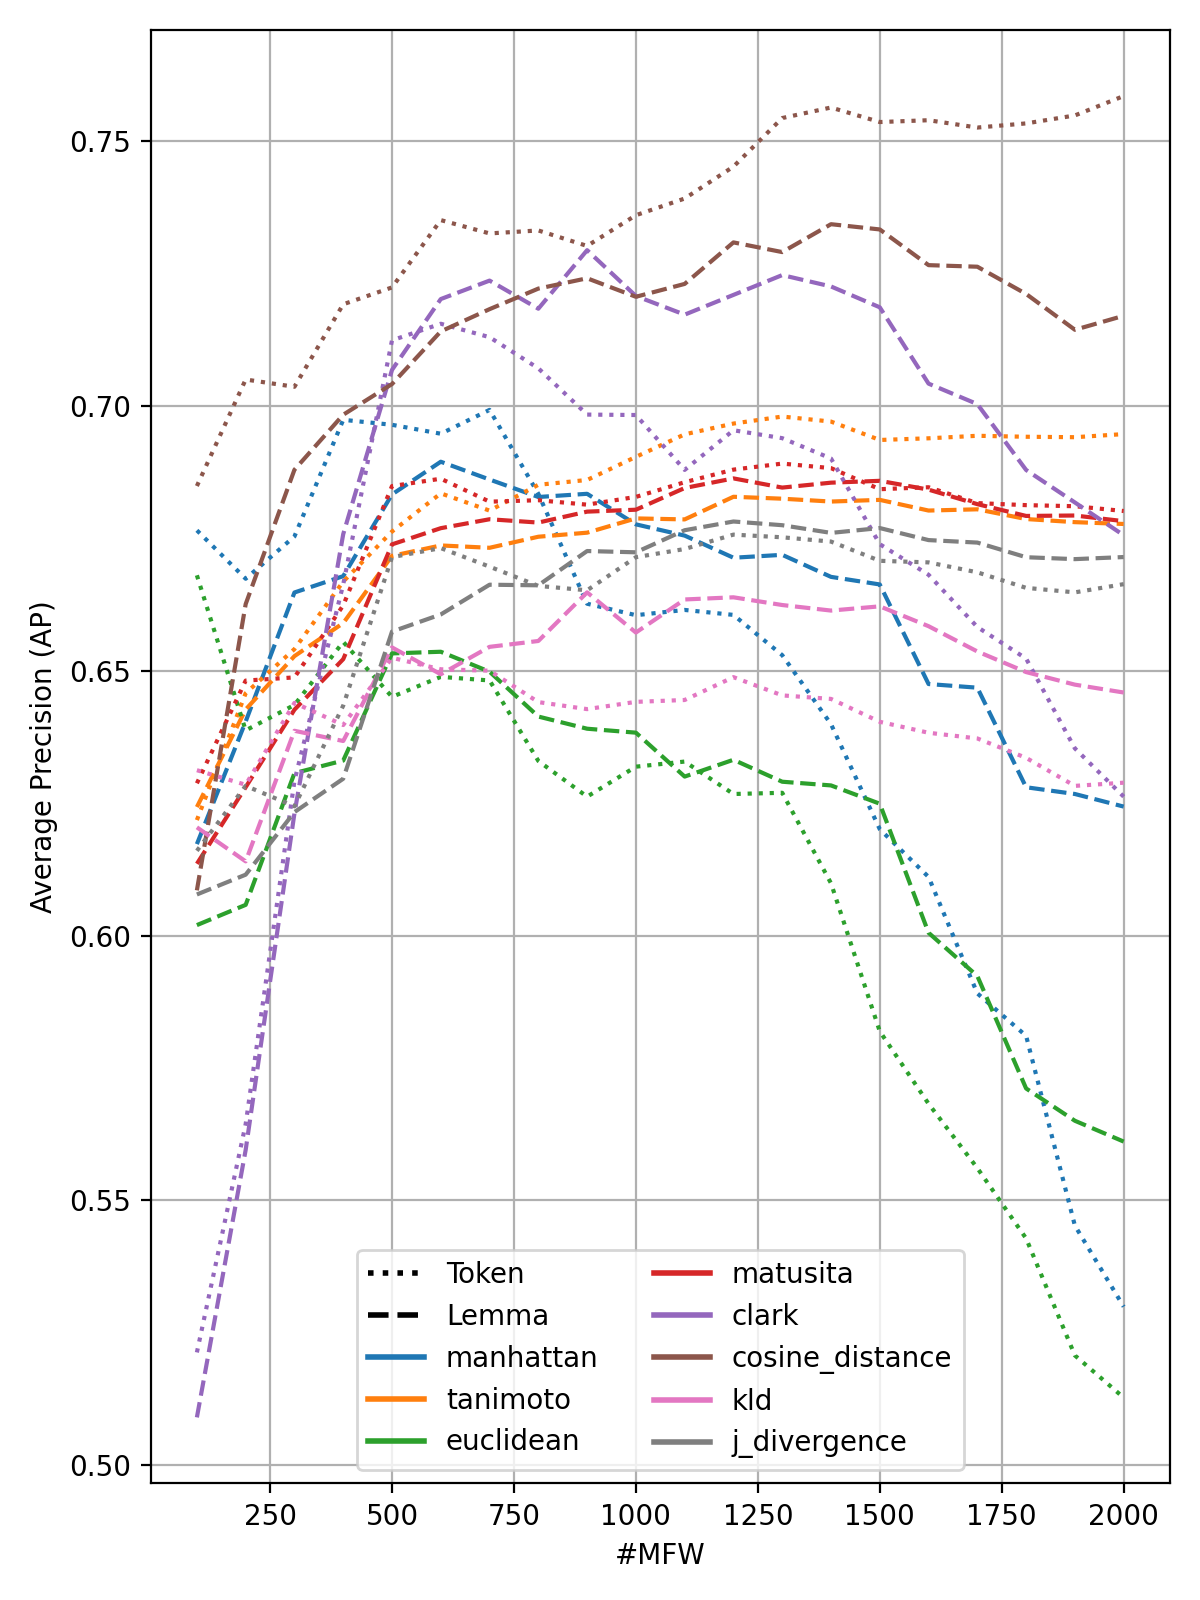
\includegraphics[width=0.9\linewidth]{img/token_vs_lemma_brunet.png}

  \vspace{0.5cm}

  \subcaption{St-Jean}
  \label{fig:token_vs_lemma_st_jean}
  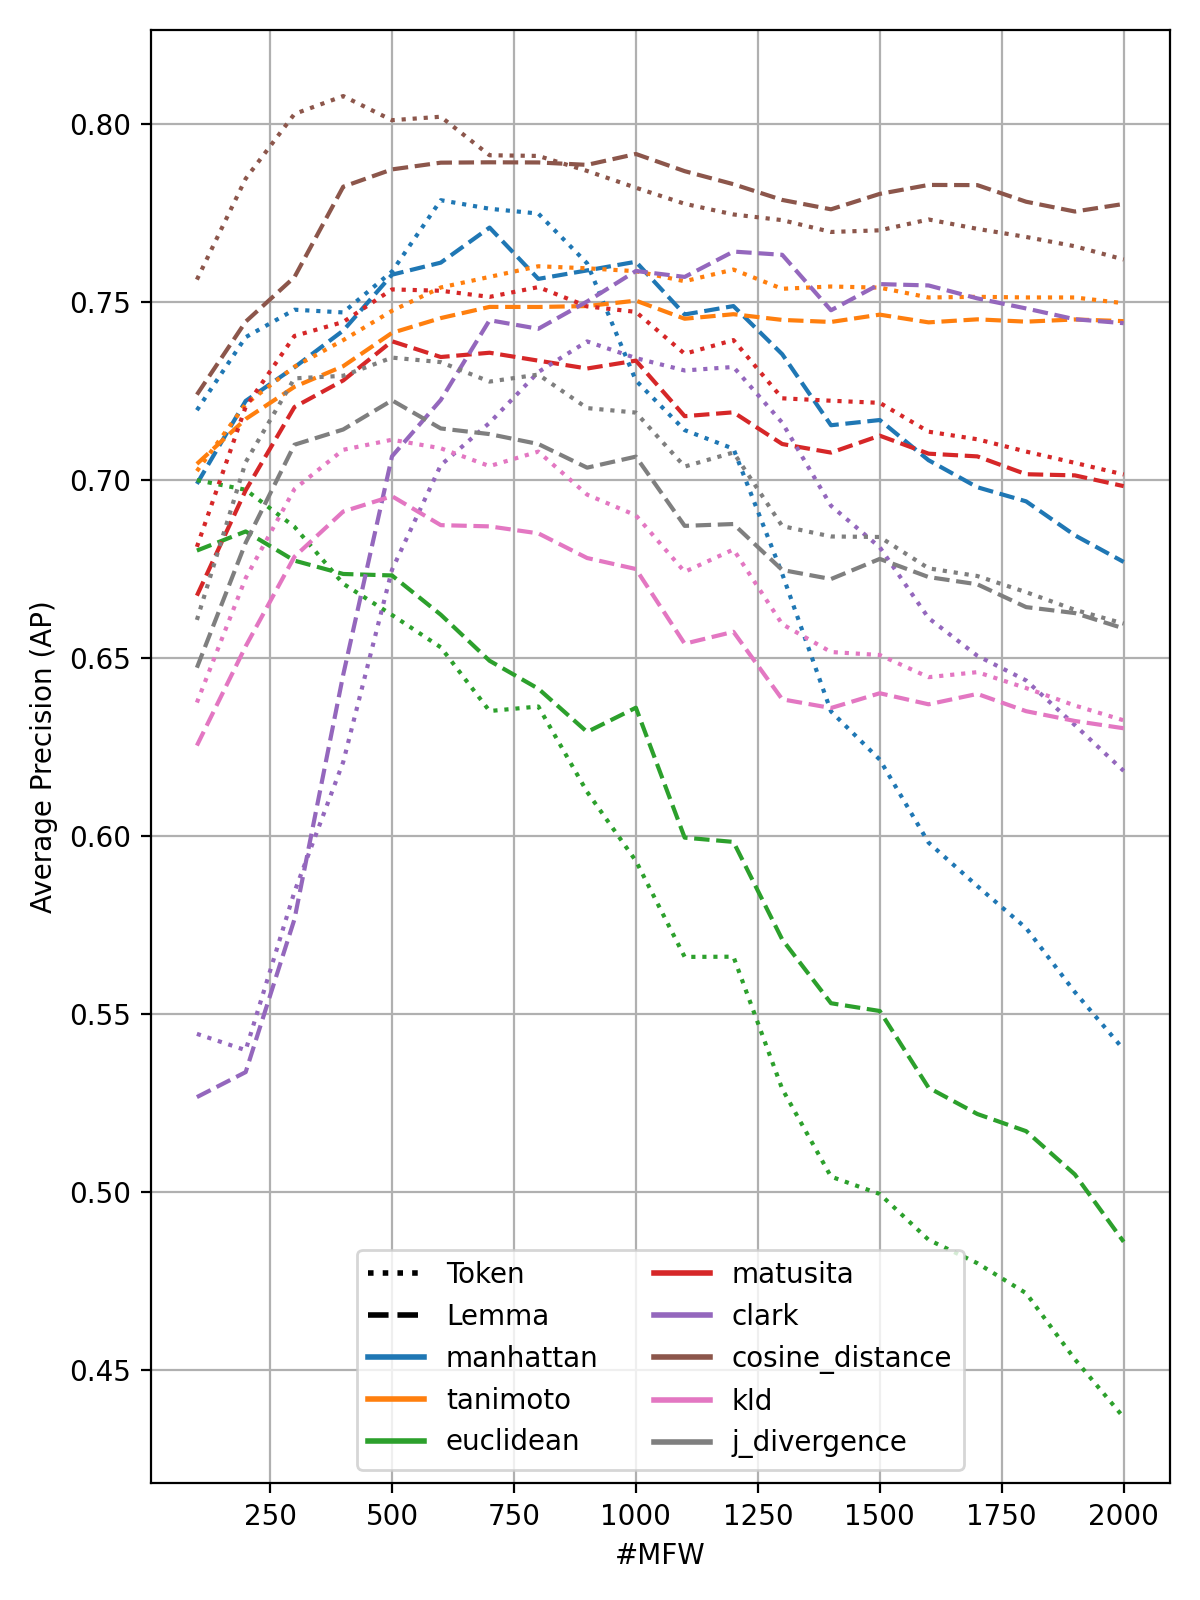
\includegraphics[width=0.9\linewidth]{img/token_vs_lemma_st_jean.png}
\end{figure}

\subsubsection{MFW Letter $n$-grams}

In this experiment the whole text is considered to create letters $n$-grams for the text representation, see Definition~\ref{def:letters_n_grams}.
As for the other experiment, the MFW approach is used to create the feature vector.
To reduce the field of the possible parameters, the experiment is split in two parts :
The first part is to find the size of the $n$ parameter of the $n$-grams, and the number of MFW.
The second is to compare the distance metrics with the previously found parameters.

One of the main drawback with this approach is that some distance metrics can have better performance on highly dimensional vectors (large MFW vector) than others, and thus this methodology does not take into account this.

\textbf{First Part}\\
For the first part, the Z-Score normalized cosine distance measure is used to compare the vectors and create the rank list.
The parameters used are: a varying MFW vector size ranging between 500 and 15000 with a step of 500 and an $n$ for the following values : $3, 4, 5, (2, 3), (3, 4), (4, 5)$.
The tuples $(a, b)$ correspond to both $a$-grams and $b$-grams in the same text representation.

The number of different $n$-grams is assumed to be larger than the vocabulary of the texts, thus the importance of having a larger vector when dealing with long texts such as the literature datasets.
When considering letters $n$-grams the text representation increases approximately by a factor of $t$, with $t$ being the average token length.
The average token size for the literature dataset is displayed Table~\ref{tab:lit_corpora} in Chapter~\ref{sec:definitions_and_corpora}, and is around $4$ characters.
To avoid having too large text representation, a possible idea is to remove the hapax legomena (tokens appearing only once in the corpus) before applying the $n$-grams algorithm.
This method can also be generalized to remove words appearing less than $x$ times.
This pruning approach was explored in~\cite{kocher_linking} but was not used in this study.

Figure~\ref{fig:letter_ngrams} show the results of the first part of the experiment on the Oxquarry dataset (\ref{fig:letter_ngrams_oxquarry}), Brunet (\ref{fig:letter_ngrams_brunet}) and St-Jean (\ref{fig:letter_ngrams_st_jean}).
The trends seem to indicate that a lower $n$ value converge with lower MFW vector size but reach a maximal value faster.
With $3$-grams, $\sim 3000-4000$-MFW give good results on both datasets with this distance metric.
On the Brunet dataset, after reaching the maximal average precision at $\sim 4000$-MFW, a larger number of frequent words decrease the precision until reaching the maximal number of different $3$-grams at $\sim 6500$-MFW, which is not the case on Oxquarry.
On St-Jean, the $3$-grams and $(2,3)$-grams do not reach a high average precision with a low number of MFW like for the Brunet and Oxquarry.
$4$-grams also can be efficient but require a larger MFW vector, around $\sim 4000$-MFW give good result for both Brunet and St-Jean but on Oxquarry it requires around $\sim 8000$ to have similar results as the $3000$ $3$-grams.
For the first part, the retained parameters for the $n$-grams text representation are the $3$-grams with $3000$-MFW and $4$-grams with $8000$-MFW.

\begin{figure}
  \caption{Letters $n$-grams representation over number of MFW with different $n$}
  \label{fig:letter_ngrams}

  \subcaption{Oxquarry}
  \label{fig:letter_ngrams_oxquarry}
  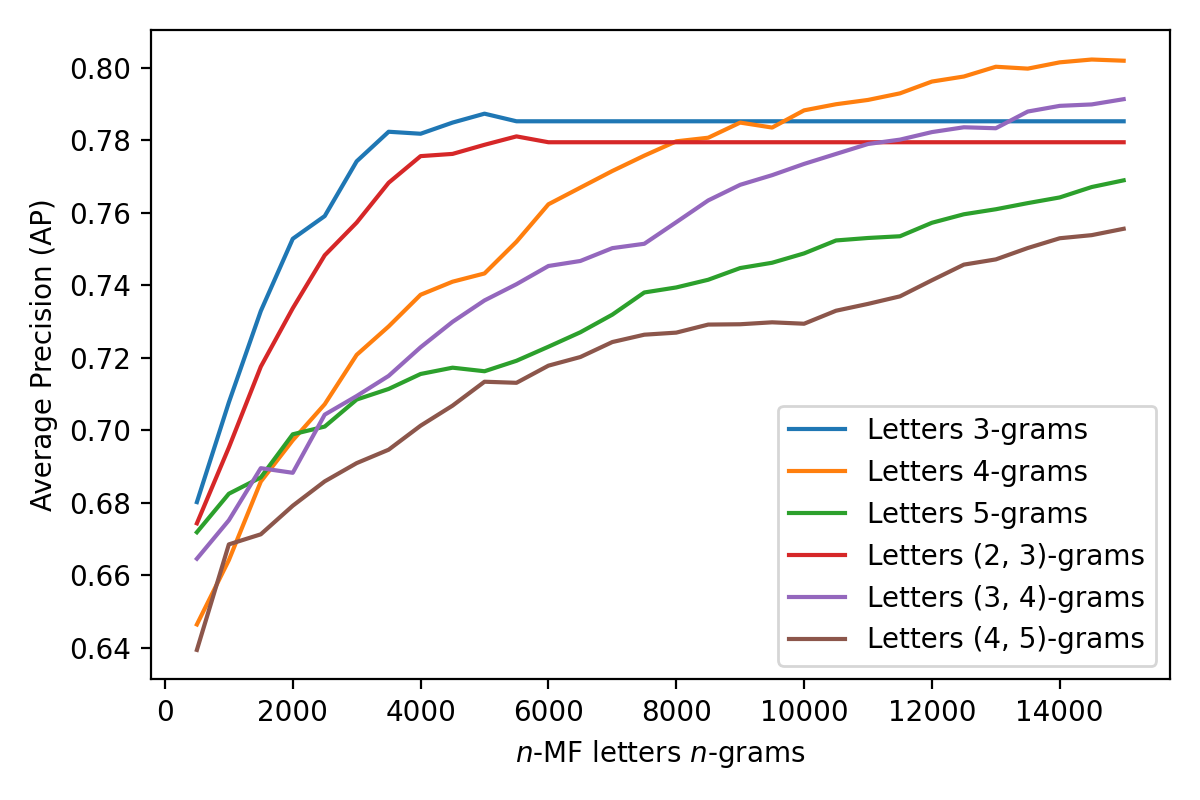
\includegraphics[width=\linewidth]{img/letter_ngrams_oxquarry.png}

  \vspace{0.5cm}

  \subcaption{Brunet}
  \label{fig:letter_ngrams_brunet}
  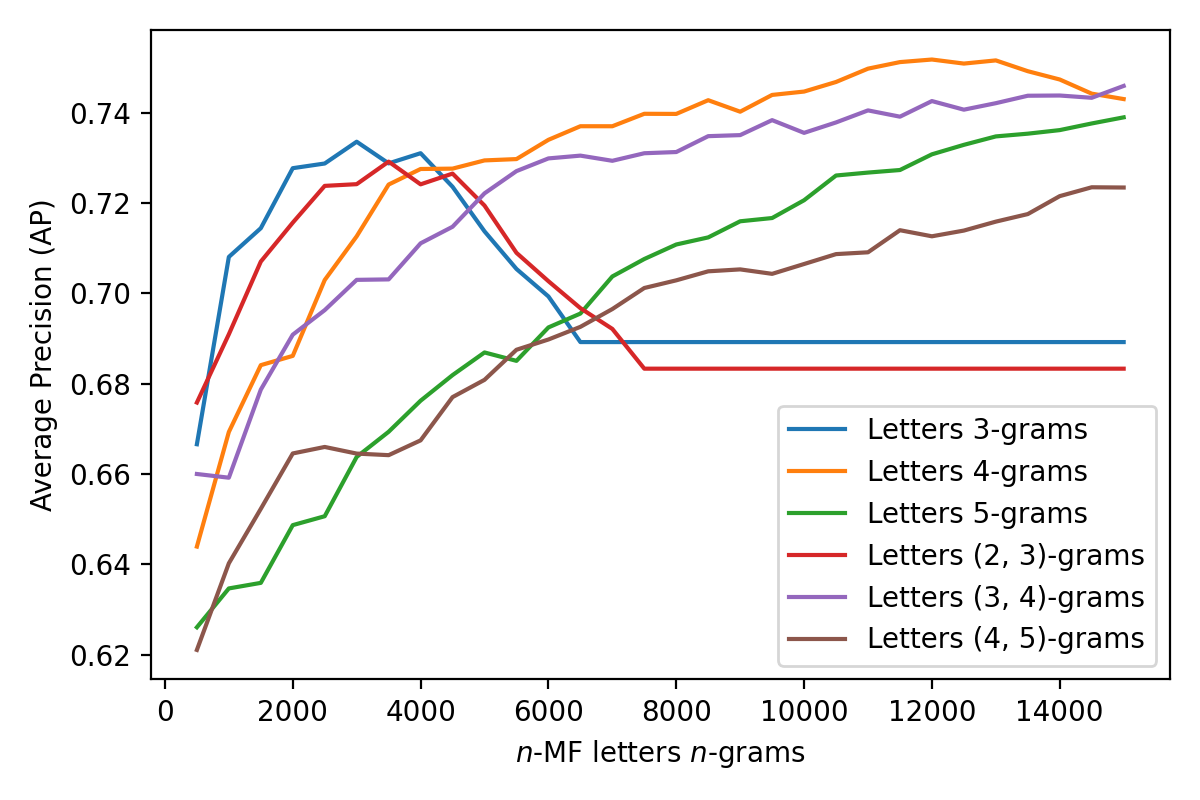
\includegraphics[width=\linewidth]{img/letter_ngrams_brunet.png}

  \vspace{0.5cm}

  \subcaption{St-Jean}
  \label{fig:letter_ngrams_st_jean}
  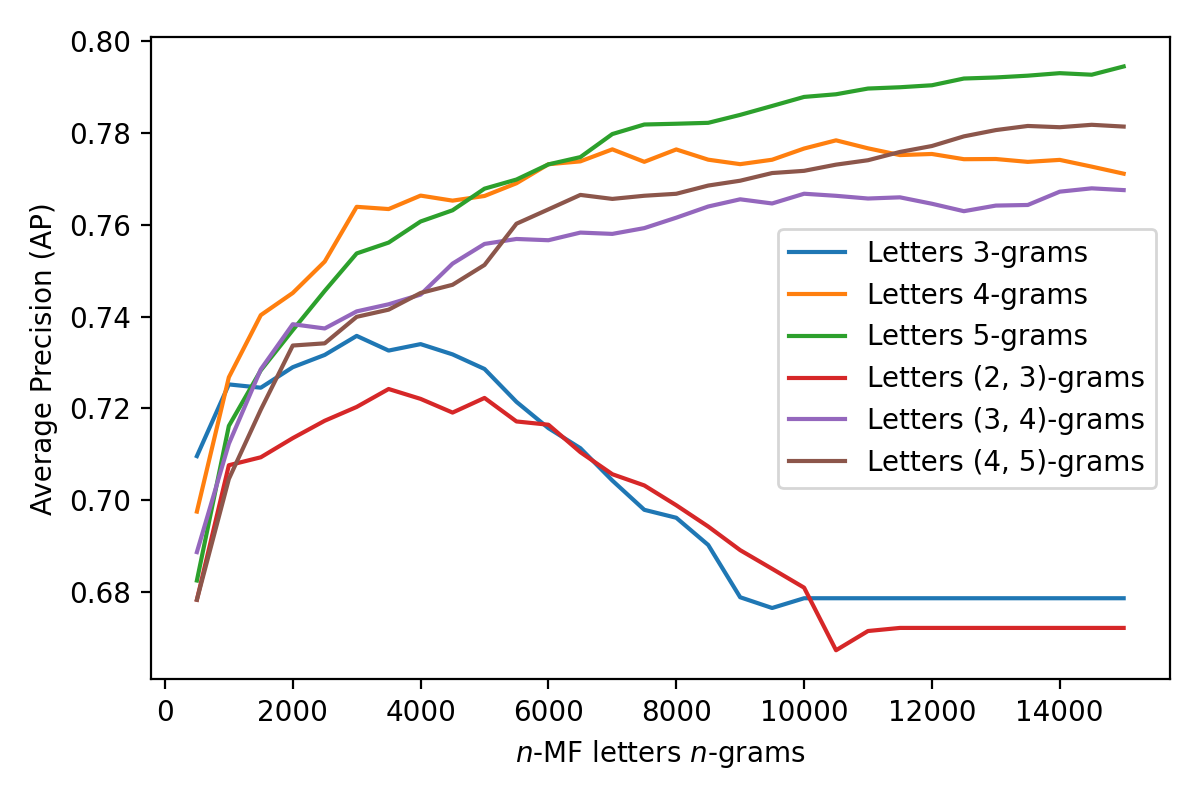
\includegraphics[width=\linewidth]{img/letter_ngrams_st_jean.png}
\end{figure}

\textbf{Second Part}\\
As stated earlier, in the second part the objective it to compare the distance metrics with the $3$-grams/$3000$-MFW and $4$-grams/$8000$-MFW.
The distance metrics used are the ones presented in Section~\ref{sec:fv_distances}.
The results for this experiment are in Table~\ref{tab:letter_ngrams}.
Since the number of MFW and the size of the $n$-grams was optimized on the Cosine distance, the results may be biased.

For the $3$-grams, the following results can be observed:
The Cosine distance give the best results.
Though, two distances metrics can compete with the Cosine distance on certain datasets with the $3$-grams approach, namely the Manhattan distance and the Clark distance.
A worth noticing results, is the Euclidean distance, which have polarized results: on Oxquarry the average precision is $0.72$ and on St-Jean only $0.47$.
Using the right distance measure can have a relative increase up to $36$\%, when comparing the worse distance metric to the best of each dataset.

For the $4$-grams approach, as for the $3$-grams the Cosine is the best measure with this configuration.
The Manhattan distance and the Clark distance also are the second choice.
The Euclidean distance have the same behaviour as for $3$-grams on the dataset.
For this configuration of $4$-grams with $8000$-MFW, using the right distance measure is less impactful than the $3$-grams approach but still can have a relative increase in performance of $28$\% when changing from the worse distance metric to the best, with these datasets.

\begin{table}
  \centering
  \caption{Average precision for $n$-grams with every metrics, on the 3 datasets (best result for the dataset in bold).}
  \label{tab:letter_ngrams}

  \subcaption{$3$-grams with $3000$-MFW}
  \begin{tabular}{l c c c}
    \toprule
    Distance metric & Oxquarry & Brunet & St-Jean \\
    \midrule
    Manhattan & \textbf{0.77} & 0.66 & 0.62 \\
    Tanimoto & 0.64 & 0.66 & 0.62 \\
    Euclidean & 0.72 & 0.63 & 0.47 \\
    Matusita & 0.60 & 0.66 & 0.58 \\
    Clark & 0.64 & \textbf{0.73} & 0.63 \\
    Cosine & \textbf{0.77} & \textbf{0.73} & \textbf{0.74} \\
    KLD & 0.57 & 0.65 & 0.54 \\
    JD & 0.58 & 0.66 & 0.56 \\
    \bottomrule
  \end{tabular}

  \vspace{0.5cm}

  \subcaption{$4$-grams with $8000$-MFW}
  \begin{tabular}{l c c c}
    \toprule
    Distance metric & Oxquarry & Brunet & St-Jean \\
    \midrule
    Manhattan & 0.76 & 0.69 & 0.73 \\
    Tanimoto & 0.68 & 0.68 & 0.68 \\
    Euclidean & 0.73 & 0.65 & 0.55 \\
    Matusita & 0.63 & 0.68 & 0.65 \\
    Clark & 0.67 & 0.72 & 0.75 \\
    Cosine & \textbf{0.78} & \textbf{0.74} & \textbf{0.78} \\
    KLD & 0.61 & 0.66 & 0.60 \\
    JD & 0.61 & 0.67 & 0.63 \\
    \bottomrule
  \end{tabular}
\end{table}

\subsubsection{MFW First letters, last letters, word $n$-grams of tokens}

In this experiment, the goal is to create 3 types of text representations of word substrings and compare them.

\begin{enumerate}
  \item
  The first representation is the $n$-first letter of each word tokens which correspond generally to the meaning of a word.
  If the word token is smaller than N, the whole word is used.
  \item
  Extract also the $n$-last letter of each word tokens, which in this case correspond to the role of the word in a sentence.
  As for the previous representation, if the word is smaller than N, the whole word is used instead.
  \item
  The in-word $n$-grams (See Definition~\ref{def:words_n_grams}), this special type of n-grams consider only $n$-grams within a word.
  This excludes every overlapping word when considering the Letters $n$-grams algorithm.
  This decision is made for this experiment such that inter-words informations can not be learned and have a fair comparison of these 3 texts representations.
\end{enumerate}

The first approach can be related to the lemma approach, the second to the POS approach and the third to a hybrid version between the letters $n$-grams and the word token text representations.
The two first representations have the same number of words as the token text representation and are a subsets of the third method.
The third representation is a subset of the Letters $n$-grams text representation.

For this experiment the only distance measure used is the Z-Score normalized Cosine distance and, for the evaluation metric, only the average precision.
The number of MFW variate for this experiment between 200 and 4000 with a step of 100.
Figure~\ref{fig:first_last_letters_ngrams} shows the results for this experiment on the three datasets (Oxquarry, Brunet, St-Jean).

In the three dataset, the 3-last letters and 3-first letters gives a lower average precision and quickly converge to an equilibrium value at around 1500 MFW.
5-letters representations tend to produce better results than 3-letters and 4-letters representation as the MFW increase.
In the Oxquarry corpus, in-word $4$-grams and in-word $5$-grams give an outstanding ~95.0\% in average precision, but is not as efficient for the Brunet dataset.
For the Brunet dataset, the 5-first letters can a good results compared to other text representations with small MFW vector size.
And for St-Jean, the 5-first letters with a small MFW vector size giv the best results.
No clear best configuration can be extracted with these results since the results are mixed across datasets, thus for this experiment, no text representation / distance measure are retained for the fusion.

\begin{figure}
  \centering
  \caption{Average precision over the MFW in the rank list generated using the Z-Score normalized Cosine distance}
  \label{fig:first_last_letters_ngrams}

  \subcaption{Oxquarry}
  \label{fig:first_last_letters_ngrams_oxquarry}
  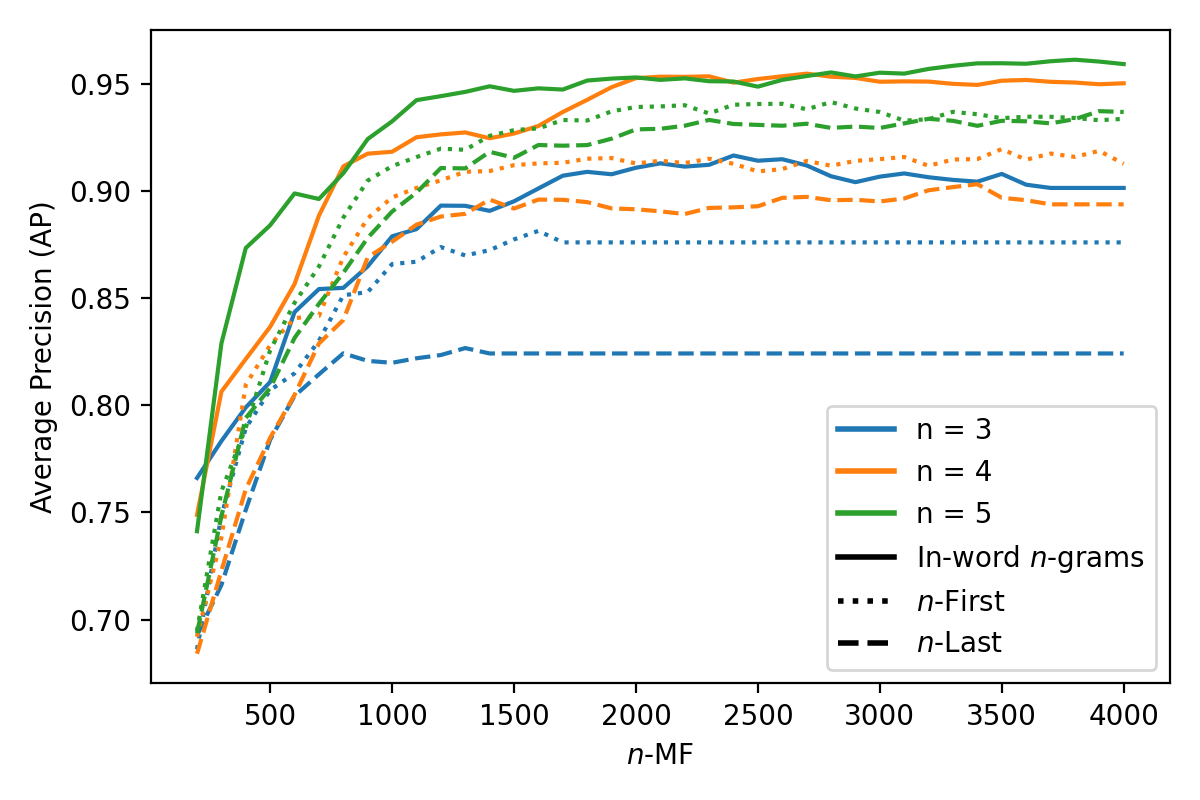
\includegraphics[width=\linewidth]{img/first_last_letters_ngrams_oxquarry.png}

  \vspace{0.5cm}

  \subcaption{Brunet}
  \label{fig:first_last_letters_ngrams_brunet}
  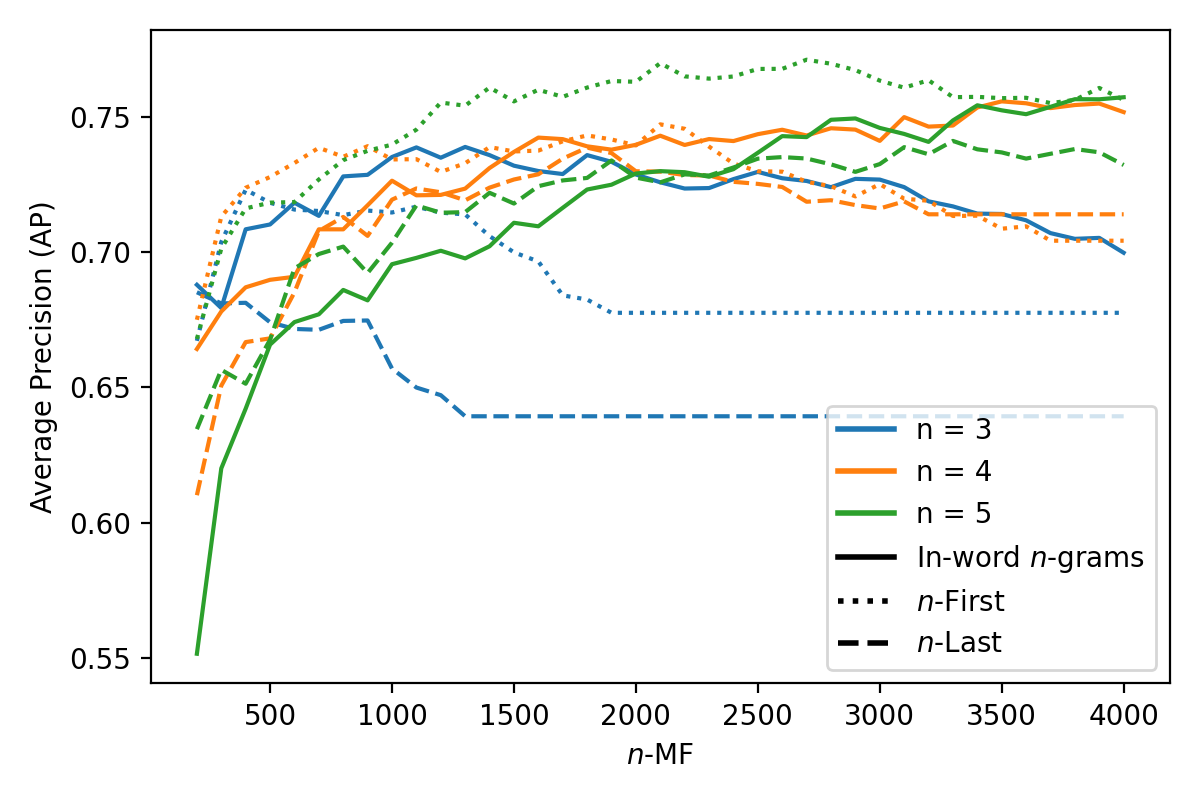
\includegraphics[width=\linewidth]{img/first_last_letters_ngrams_brunet.png}

  \vspace{0.5cm}

  \subcaption{St-Jean}
  \label{fig:first_last_letters_ngrams_st_jean}
  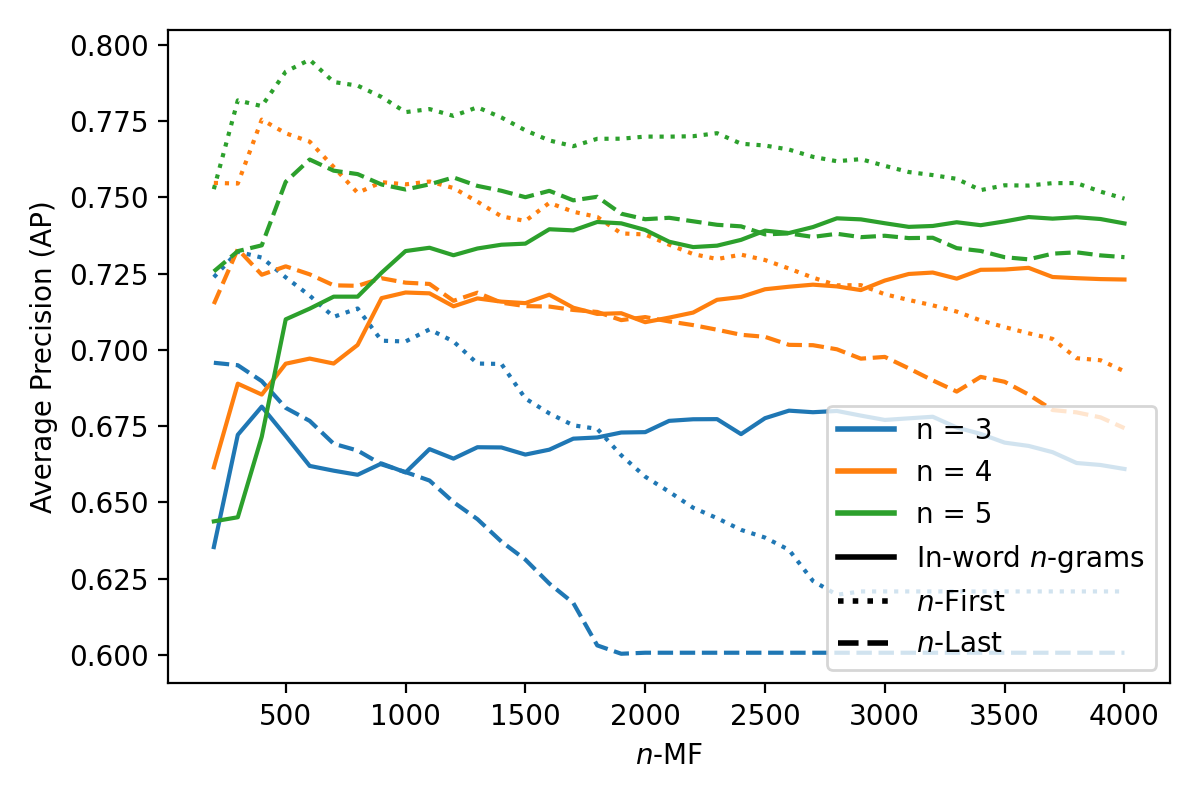
\includegraphics[width=\linewidth]{img/first_last_letters_ngrams_st_jean.png}
\end{figure}

\subsubsection{MFW POS $n$-grams}

For this experiment, short combination of POS are used to detect the style of the author.
POS $1$-grams are discarded from the experiment (equivalent of the POS frequency) since previous studies showed that POS $1$-grams tends to produce worse results then POS $2$/$3$/$4$-grams~\cite{kocher_linking}.
The St-Jean dataset have for every word a POS tag, by using these POS tags and combining them using Definition~\ref{def:letters_n_grams} to create $n$-grams/w-shingling, a new text representation is obtained.
This representation can be related to the author style sentence structure.
As for previous methods, the rank list is computed by scoring every document pairs, using the feature vector created with the MFW POS $n$-grams.
The experiment is split in two parts, the first aim to select the most convincing size of POS $n$-grams and the size of the feature vector.
The second is to compare the different distance metrics.
Keep in mind, as for the previous experiment in two parts, this experimentation methodology ignore the strength and weakness of distance measure with regard to the dimensionality of the vectors.

\textbf{First Part}\\
In this experiment, only $2$-grams, $3$-grams, $4$-grams and the combination of the $2$-grams and $3$-grams denoted: $(2, 3)$-grams is used.
The distance metric used for this part is the smoothed Z-Score normalized Cosine distance.
For this representation no clear MFW vector size is advised (in this case POS $n$-grams are considered as words in the MFW definition), the size used is between 200 and 2000 with a step of 100.
Figure~\ref{fig:pos_ngrams} show the average precision on the rank list produced by using POS $n$-grams over the number of MFW.

The two following information can be intuitively observed on this plot:
\begin{itemize}
  \item
  A more complex POS $n$-grams require more MFW to achieve its maximal effectiveness.
  In the St-Jean corpus, a total of 26 different POS are used to describe every words in the corpus.
  Which correspond to $26^2 = 676$ possible unique POS $2$-grams sequences, to $26^3 = 17,576$ POS $3$-grams and $26^4 = 456,976$ POS $4$-grams, thus $2$-grams converges and not $3$/$4$-grams.
  \item
  Like other methods, if the MFW ceiling is too high, an overfitting to less important words is possible, thus reducing the average precision.
  In Figure~\ref{fig:pos_ngrams} the POS 2-grams clearly have a drop in average precision after $\sim 250$-MFW.
\end{itemize}

Using the smoothed Z-Score Cosine distance, the most appropriate configuration for the POS $n$-grams text representation on St-Jean seem to be $250$-MFW POS $2$-grams and $1000$-MFW POS $3$-grams.

\begin{figure}
  \centering
  \caption{Average precision over the MFW in the rank list generated using the Z-Score normalized Cosine distance on St-Jean POS n-grams text representation.}
  \label{fig:pos_ngrams}
  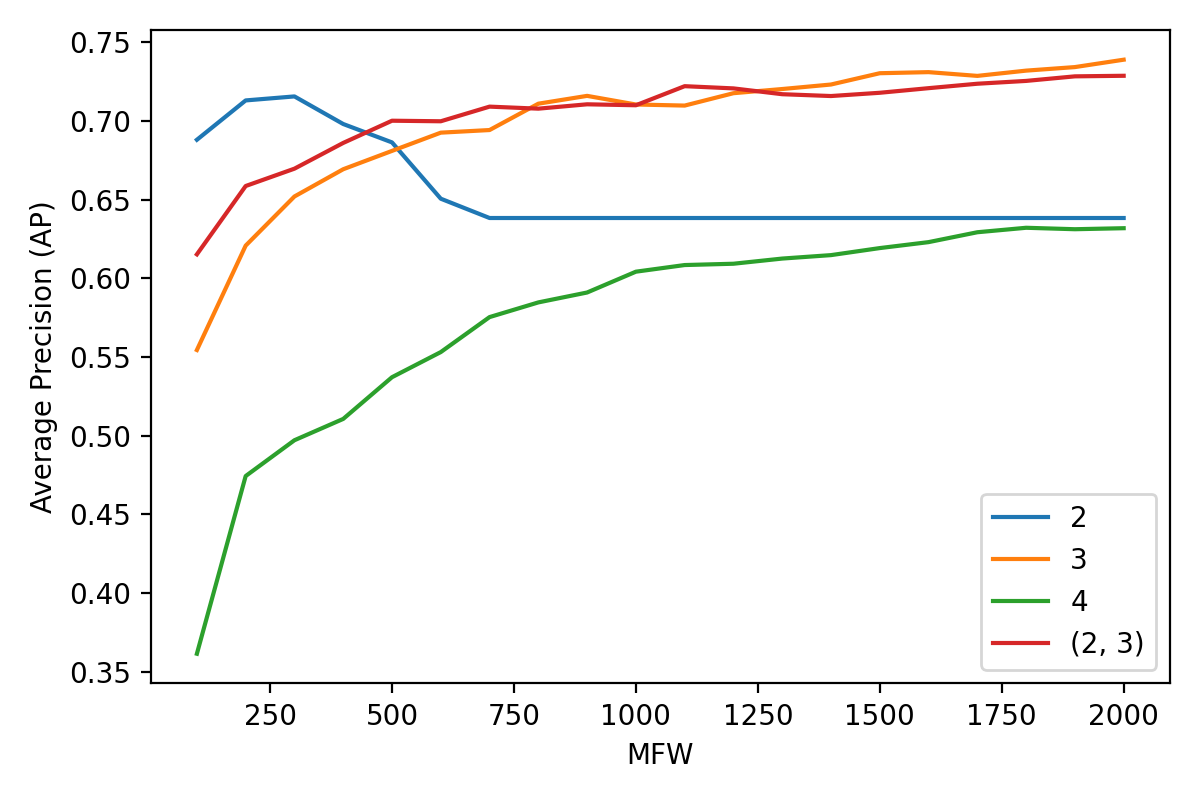
\includegraphics[width=\linewidth]{img/pos_ngrams.png}
\end{figure}

\textbf{Second Part}\\
In this second part, the goal is to find the most appropriate distance metric for the POS $n$-grams text representation, with the configuration retained in the first part.
After running with these parameters on every proposed distance metrics, Table~\ref{tab:pos_ngrams} shows a resume of the experiment.

When considering POS $n$-grams as text representation on the St-Jean dataset, over all the best distance metrics are Manhattan, Matusita, Cosine distance.
The Clark distance, give overall the worse results, even though in other text representation, this metric was giving the best results.
Using an optimized distance metric can increase the average precision by up to $36$\% in average with this dataset and this text representation.

The retained configurations using the POS $n$-grams text representation is the $250$-MFW POS $2$-grams using the smoothed Z-Score Cosine Distance and $1000$-MFW POS $3$-grams using the smoothed Z-Scored Manhattan distance.

\begin{table}
  \centering
  \caption{Average precision for every distance metrics with the POS $n$-grams representation on St-Jean ($n$-grams/$n$-MFW)}
  \label{tab:pos_ngrams}
  \begin{tabular}{l c c c}
    \toprule
                    & \multicolumn{2}{c}{$n$-grams/$n$-MFW} \\
    Distance metric & $2$/$250$ & $3$/$1000$ \\
    \midrule
    Manhattan & 0.70 & \textbf{0.75} \\
    Tanimoto & 0.67 & 0.72 \\
    Euclidean & 0.69 & 0.72 \\
    Matusita & 0.70 & 0.73 \\
    Clark & 0.50 & 0.60 \\
    Cosine & \textbf{0.73} & 0.71 \\
    KLD & 0.68 & 0.70 \\
    JD & 0.69 & 0.73 \\
    \bottomrule
  \end{tabular}
\end{table}

\subsubsection{Every vocabulary tokens in the feature vectors}

Previously the MF (most frequent) method was proposed to limit the words used to only the most frequents in the vocabulary of a corpus.
This experiment aim to show the importance of limiting the words used when creating the vector representing the document.
Three approach are compared, the first use the whole corpus vocabulary to create the feature vector, denoted \textit{every token}.
In the second, every token appearing more than once are used to create the vector, denoted \textit{without hapax legomena}.
And for the last, the vector contain the 750 most frequent words, denoted \textit{750-MFW}.

The eight proposed distance measures are evaluated for the three approach using the average precision metric on the three literature corpora.
To understand more easily the results for the three approach, the \textit{every token} approach is used as a baseline from where the average precision gain is computed.

Table~\ref{tab:baseline_every_token} show the average precision baseline using the \textit{every token} approach.
Table~\ref{tab:gain_without_hapax_legomena} and Table~\ref{tab:gain_750_mfw} show the gain over the baseline for the \textit{without hapax legomena} approach and \textit{750-MFW} approach respectively.

When looking at the baseline : the Manhattan, Euclidean and Clark distance measure have a poor average precision, all are below 0.3 in average.
The other metric have average to good results which range from 0.58 for the KLD to 0.79 with the Cosine distance.
The Cosine distance with \textit{every token} reach a 0.91 average precision for the Oxquarry corpus.
When removing hapax legomena, for most distance metrics the gain in average precision is limited, except for the Clark distance where the mean average precision rise from 0.3 to 0.5.
After limiting to the 750-MFW, the Manhattan, Euclidean and Clark distance, the ones that had poor results for the baseline increase their average precision by around 48\% which correspond to an average precision of 0.71, 0.63 and 0.78 respectively, which makes them in the same range as the other metrics in the baseline.
Across every metric and dataset, removing hapax legomena increase the average precision in average by 0.04, and limiting to the 750-MFW by 0.21.
This clearly indicate the importance of limiting the size of the vector.

From this experiment, each distance metric can be placed in one of the two following categories : the ones sensible to noisy vectors, the ones not sensible.
In the first category are : Manhattan, Clark and Euclidean, in the second : Cosine, Matusita and Tanimoto.
As for KLD and JD, they are nor in the first nor the second since both of them had a small gain in regard to the Oxquarry corpus but larger gain for the St-Jean dataset.
Further, test are required to classify these distance metrics.

\begin{table}
  \centering
  \caption{Rank lists average precision depending on the number of token used}

  \subcaption{Baseline: \textit{every token}}
  \label{tab:baseline_every_token}
  \begin{tabular}{l r r r|r}
    \toprule
    Metric & Oxquarry & Brunet & St-Jean & Mean \\
    \midrule
    Manhattan & 0.27 & 0.21 & 0.17 & 0.22 \\
    Tanimoto  & 0.63 & 0.65 & 0.70 & 0.66 \\
    Euclidean & 0.19 & 0.19 & 0.08 & 0.15 \\
    Matusita  & 0.61 & 0.63 & 0.62 & 0.62 \\
    Clark     & 0.40 & 0.28 & 0.21 & 0.30 \\
    Cosine    & 0.91 & 0.73 & 0.73 & 0.79 \\
    KLD       & 0.58 & 0.59 & 0.56 & 0.58 \\
    JD        & 0.59 & 0.63 & 0.59 & 0.60 \\
    \midrule
    Mean      & 0.52 & 0.49 & 0.46 & 0.49 \\
    \bottomrule
  \end{tabular}

  \vspace{0.5cm}

  \subcaption{Gain \textit{without hapax legomena} over baseline}
  \label{tab:gain_without_hapax_legomena}
  \begin{tabular}{l r r r|r}
    \toprule
    Metric & Oxquarry & Brunet & St-Jean & Mean \\
    \midrule
    Manhattan & +0.10 & +0.05 & +0.02 & +0.06 \\
    Tanimoto  & -0.00 & +0.01 & +0.00 & +0.01 \\
    Euclidean & +0.11 & +0.01 & +0.00 & +0.04 \\
    Matusita  & -0.01 & +0.01 & -0.01 & -0.00 \\
    Clark     & +0.19 & +0.16 & +0.25 & +0.20 \\
    Cosine    &  0.02 & -0.02 & -0.02 & -0.01 \\
    KLD       & -0.02 & +0.02 & -0.01 & -0.00 \\
    JD        & -0.01 & +0.01 & -0.02 & -0.01 \\
    \midrule
    Mean      & +0.05 & +0.03 & +0.03 & +0.04 \\
    \bottomrule
  \end{tabular}

  \vspace{0.5cm}

  \subcaption{Gain \textit{750-MFW} over baseline}
  \label{tab:gain_750_mfw}
  \begin{tabular}{l r r r|r}
    \toprule
    Metric & Oxquarry & Brunet & St-Jean & Mean \\
    \midrule
    Manhattan & +0.40 & +0.47 & +0.59 & +0.49 \\
    Tanimoto  & +0.00 & +0.03 & +0.05 & +0.03 \\
    Euclidean & +0.43 & +0.45 & +0.57 & +0.48 \\
    Matusita  & +0.02 & +0.05 & +0.12 & +0.06 \\
    Clark     & +0.49 & +0.44 & +0.53 & +0.48 \\
    Cosine    & -0.02 & -0.02 & +0.06 & +0.01 \\
    KLD       & +0.02 & +0.07 & +0.12 & +0.07 \\
    JD        & +0.02 & +0.04 & +0.12 & +0.06 \\
    \midrule
    Mean      & +0.17 & +0.19 & +0.27 & +0.21 \\
    \bottomrule
  \end{tabular}
\end{table}

\subsubsection{Compression based distances}

This experiment try to compare the three proposed compression algorithm (GZip, BZip2, LZMA) for the compression based distance ranking.
For each algorithm and for each document, the size after compression is computed, as well as the concatenation of every document pairs.
Using these sizes and the NCD or CBC distance metrics (ref. Section~\ref{sec:compression_based_distances}), the rank list is evaluated.
This experiment is run on the three corpora three times to have a better approximation of the run time.
The results in terms of efficiency of the resulting rank list are shown in Table~\ref{tab:compression_evaluation_results}.
The average time of the three runs are in Table~\ref{tab:compression_evaluation_times} when run on an Intel(R) Core(TM) i7-5820K CPU @ 3.30GHz.

GZip seem to be giving the worse results on every dataset with an absolute average AP of $\sim -0.20$ in compared to LZMA and BZip2.
LZMA gives the best results on every dataset tested, but BZip2 have close results.

The Cosine-based compression distance (CBC) tend to give better results over the normalized compression distance (NCD).
In terms of time complexity BZip2 is the fastest algorithm of the 3 proposed, LZMA is $\sim ~5-6$ times slower than BZip2, and GZip slower than BZip2 by around $\sim 5-20$\%.
No significant time differences is recorded between the NCD and CBC distance measures, since the greatest complexity reside in the compression algorithm.
Even though LZMA algorithm give the best results, the configuration retained for the compression based distance is the BZip2 with the Cosine based compression distance, since it gives relative good results in a short amount of time.
Previous study show that the distance measure choice was more impactful than the choice of the compression algorithm in the regarding the quality of the results~\cite{comparing_compression}.
Our results tend to indicate the opposite, ref. Table~\ref{tab:compression_evaluation_results}.
The distance measures does not impact a lot the quality of the results, but the compression algorithm does.
This difference may be cause by the difference of compression algorithm used.

For this text representation, the retained configuration is the BZip2 algorithm with the CBC distance measure.
The Bzip2 was selected even though LZMA give slightly better results, due to the huge difference in run time.

\begin{table}
  \centering
  \caption{Evaluation of the different compression algorithm and distance metrics using Average Precision (AP), R-Precision (RP) and High Precision (HP)}
  \label{tab:compression_evaluation_results}

  \subcaption{Oxquarry}
  \label{tab:compression_evaluation_oxquarry}
  \begin{tabular}{l c c}
    \toprule
    AP/RPrec/HPrec & NCD          & CBC \\
    \midrule
    Bzip2          & 0.77/0.68/69 & 0.79/0.69/74 \\
    GZip           & 0.62/0.56/41 & 0.64/0.56/43 \\
    LZMA           & 0.81/0.70/82 & 0.84/0.73/85 \\
    \bottomrule
  \end{tabular}

  \vspace{0.5cm}

  \subcaption{Brunet}
  \label{tab:compression_evaluation_brunet}
  \begin{tabular}{l c c}
    \toprule
    AP/RPrec/HPrec & NCD          & CBC \\
    \midrule
    Bzip2          & 0.76/0.70/25 & 0.76/0.70/25 \\
    GZip           & 0.61/0.53/24 & 0.60/0.52/23 \\
    LZMA           & 0.78/0.73/27 & 0.79/0.73/31 \\
    \bottomrule
  \end{tabular}

  \vspace{0.5cm}

  \subcaption{St-Jean}
  \label{tab:compression_evaluation_st_jean}
  \begin{tabular}{l c c}
    \toprule
    AP/RPrec/HPrec & NCD           & CBC \\
    \midrule
    Bzip2          & 0.70/0.63/214 & 0.70/0.62/219 \\
    GZip           & 0.45/0.44/54  & 0.42/0.42/56 \\
    LZMA           & 0.71/0.63/241 & 0.71/0.62/214 \\
    \bottomrule
  \end{tabular}
\end{table}

\begin{table}
  \centering
  \caption{Average run time for the rank list computation with the different compression algorithm and distance metrics}
  \label{tab:compression_evaluation_times}

  \subcaption{Oxquarry}
  \label{tab:compression_evaluation_time_oxquarry}
  \begin{tabular}{l c c}
    \toprule
    Time      & NCD   & CBC \\
    \midrule
    Bzip2     & 12.7s & 12.7s \\
    GZip      & 15.0s & 14.9s \\
    LZMA      & 69.0s & 68.8s \\
    \bottomrule
  \end{tabular}

  \vspace{0.5cm}

  \subcaption{Brunet}
  \label{tab:compression_evaluation_time_brunet}
  \begin{tabular}{l c c}
    \toprule
    Time      & NCD   & CBC \\
    \midrule
    Bzip2     & 8.4s & 8.4s \\
    GZip      & 8.8s & 8.9s \\
    LZMA      & 46.6s & 46.8s \\
    \bottomrule
  \end{tabular}

  \vspace{0.5cm}

  \subcaption{St-Jean}
  \label{tab:compression_evaluation_time_st_jean}
  \begin{tabular}{l c c}
    \toprule
    Time      & NCD    & CBC \\
    \midrule
    Bzip2     & 198.9s  & 198.4s \\
    GZip      & 211.3s  & 214.5s \\
    LZMA      & 1046.3s & 1052.0s \\
    \bottomrule
  \end{tabular}
\end{table}

\subsubsection{Summary of the retained individual rank lists}

For the next experiments, medium to high quality rank list are required.
The previous experiments tried to find some good rank list produced across different text representation.
The retained text representations are presented in Table~\ref{tab:9rl}.
Four of them are using the MFW tokens, two MFW tokens n-grams, one the compression and two the MFW POS n-grams.
The complete evaluation of the rank list produced on these text representation for the three literary corpora are presented in Section~\ref{sec:annex_retained_text_representation} in annex.

\begin{table*}
  \centering
  \caption{Retained text representation, text representation with a star (*) are only used for the St-Jean dataset}
  \label{tab:9rl}
  \begin{tabular}{c l l c}
    \toprule
    Id &
    Text representation &
    Distance measure &
    Z-Score \\
    \midrule
    0 & $750$-MFW tokens & Cosine Distance & x\\
    1 & $750$-MFW tokens & Clark & \\
    2 & $750$-MFW tokens & Manhattan & x\\
    3 & $750$-MFW tokens & Tanimoto & \\
    4 & $3000$-MFW tokens $3$-grams & Cosine distance & x\\
    5 & $8000$-MFW tokens $4$-grams & Cosine distance & x\\
    6 & BZip2 compression & CBC distance & \\
    *7 & $250$-MFW POS $2$-grams & Cosine distance & x\\
    *8 & $1000$-MFW POS $3$-grams & Manhattan distance & x\\
    \bottomrule
  \end{tabular}
\end{table*}
